\documentclass[10pt, compress]{beamer}

\usetheme[numbering=fraction, progressbar=none, titleformat=smallcaps, sectionpage=none]{metropolis}
\usepackage{booktabs}
\usepackage{array}
\usepackage{listings}
\usepackage{graphicx}
\usepackage[english]{babel}
\usepackage[scale=2]{ccicons}
\usepackage{url}
\usepackage{relsize}
\usepackage{wasysym}

\usepackage{pgfplots}
\usepgfplotslibrary{dateplot}

\lstset{ %
  backgroundcolor={},
  basicstyle=\ttfamily\footnotesize,
  breakatwhitespace=true,
  breaklines=true,
  captionpos=n,
  commentstyle=\color{orange},
  escapeinside={\%*}{*)},
  extendedchars=true,
  frame=n,
  keywordstyle=\color{orange},
  language=C++,
  rulecolor=\color{black},
  showspaces=false,
  showstringspaces=false,
  showtabs=false,
  stepnumber=2,
  stringstyle=\color{gray},
  tabsize=2,
  keywords={thrust,plus,device_vector, copy,transform,begin,end, copyin,
  copyout, acc, \_\_global\_\_, void, int, float, main, threadIdx, blockIdx,
  blockDim, if, else, malloc, NULL, cudaMalloc, cudaMemcpy, cudaSuccess,
  cudaGetLastError, cudaDeviceSynchronize, cudaFree, cudaMemcpyDeviceToHost,
  cudaMemcpyHostToDevice, const, data, independent, kernels, loop,
  fprintf, stderr, cudaGetErrorString, EXIT_FAILURE, for, dim3},
  otherkeywords={::, \#pragma, \#include, <<<,>>>, \&, \*, +, -, /, [, ], >, <}
}

\renewcommand*{\UrlFont}{\ttfamily\smaller\relax}

\graphicspath{{../img/}}

\title{Introduction to GPU Programming \\ with the CUDA Platform}
\author{\footnotesize Marco Dimas Gubitoso \\ {\scriptsize gubi@ime.usp.br}}
\institute{
\includegraphics[height=2cm]{imelogo}\\[0.2cm] Instituto de Matemática e Estatística \\ Universidade de São Paulo}
\date{\scriptsize 4th INFIERI, 2017}

\begin{document}

\part{Part I}

\maketitle

\section{Introduction}

\subsection{About}

\begin{frame}
    \frametitle{About}
    \footnotesize
    \begin{columns}[T,onlytextwidth]
        \column{0.5\textwidth}
        \begin{center}
            
\includegraphics[width=.42\textwidth]{pedro}

            Pedro Bruel

            \alert{phrb}@ime.usp.br
        \end{center}

        \column{0.5\textwidth}
        \begin{center}
            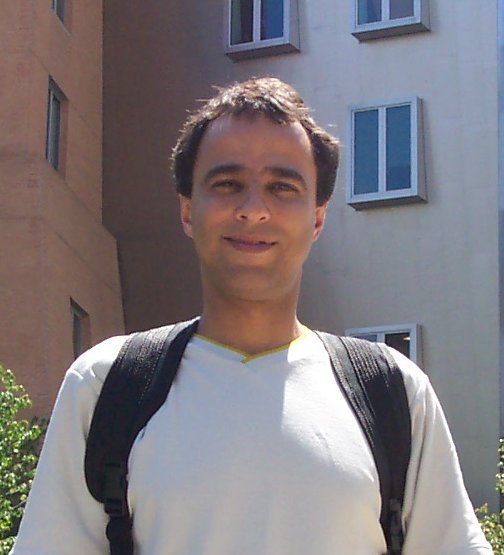
\includegraphics[width=.37\textwidth]{alfredo}

            Alfredo Goldman

            \alert{gold}@ime.usp.br
        \end{center}

    \end{columns}

    \begin{center}
        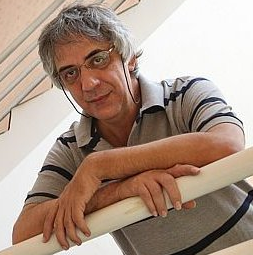
\includegraphics[width=.18\textwidth]{gubi}

        Marco Dimas Gubitoso

        \alert{gubi}@ime.usp.br
    \end{center}
\end{frame}

\subsection{Justification}

\begin{frame}
    \frametitle{Hardware Acceleration}
    Percentage of systems with accelerators in the \textit{Top500}:

    \begin{center}
    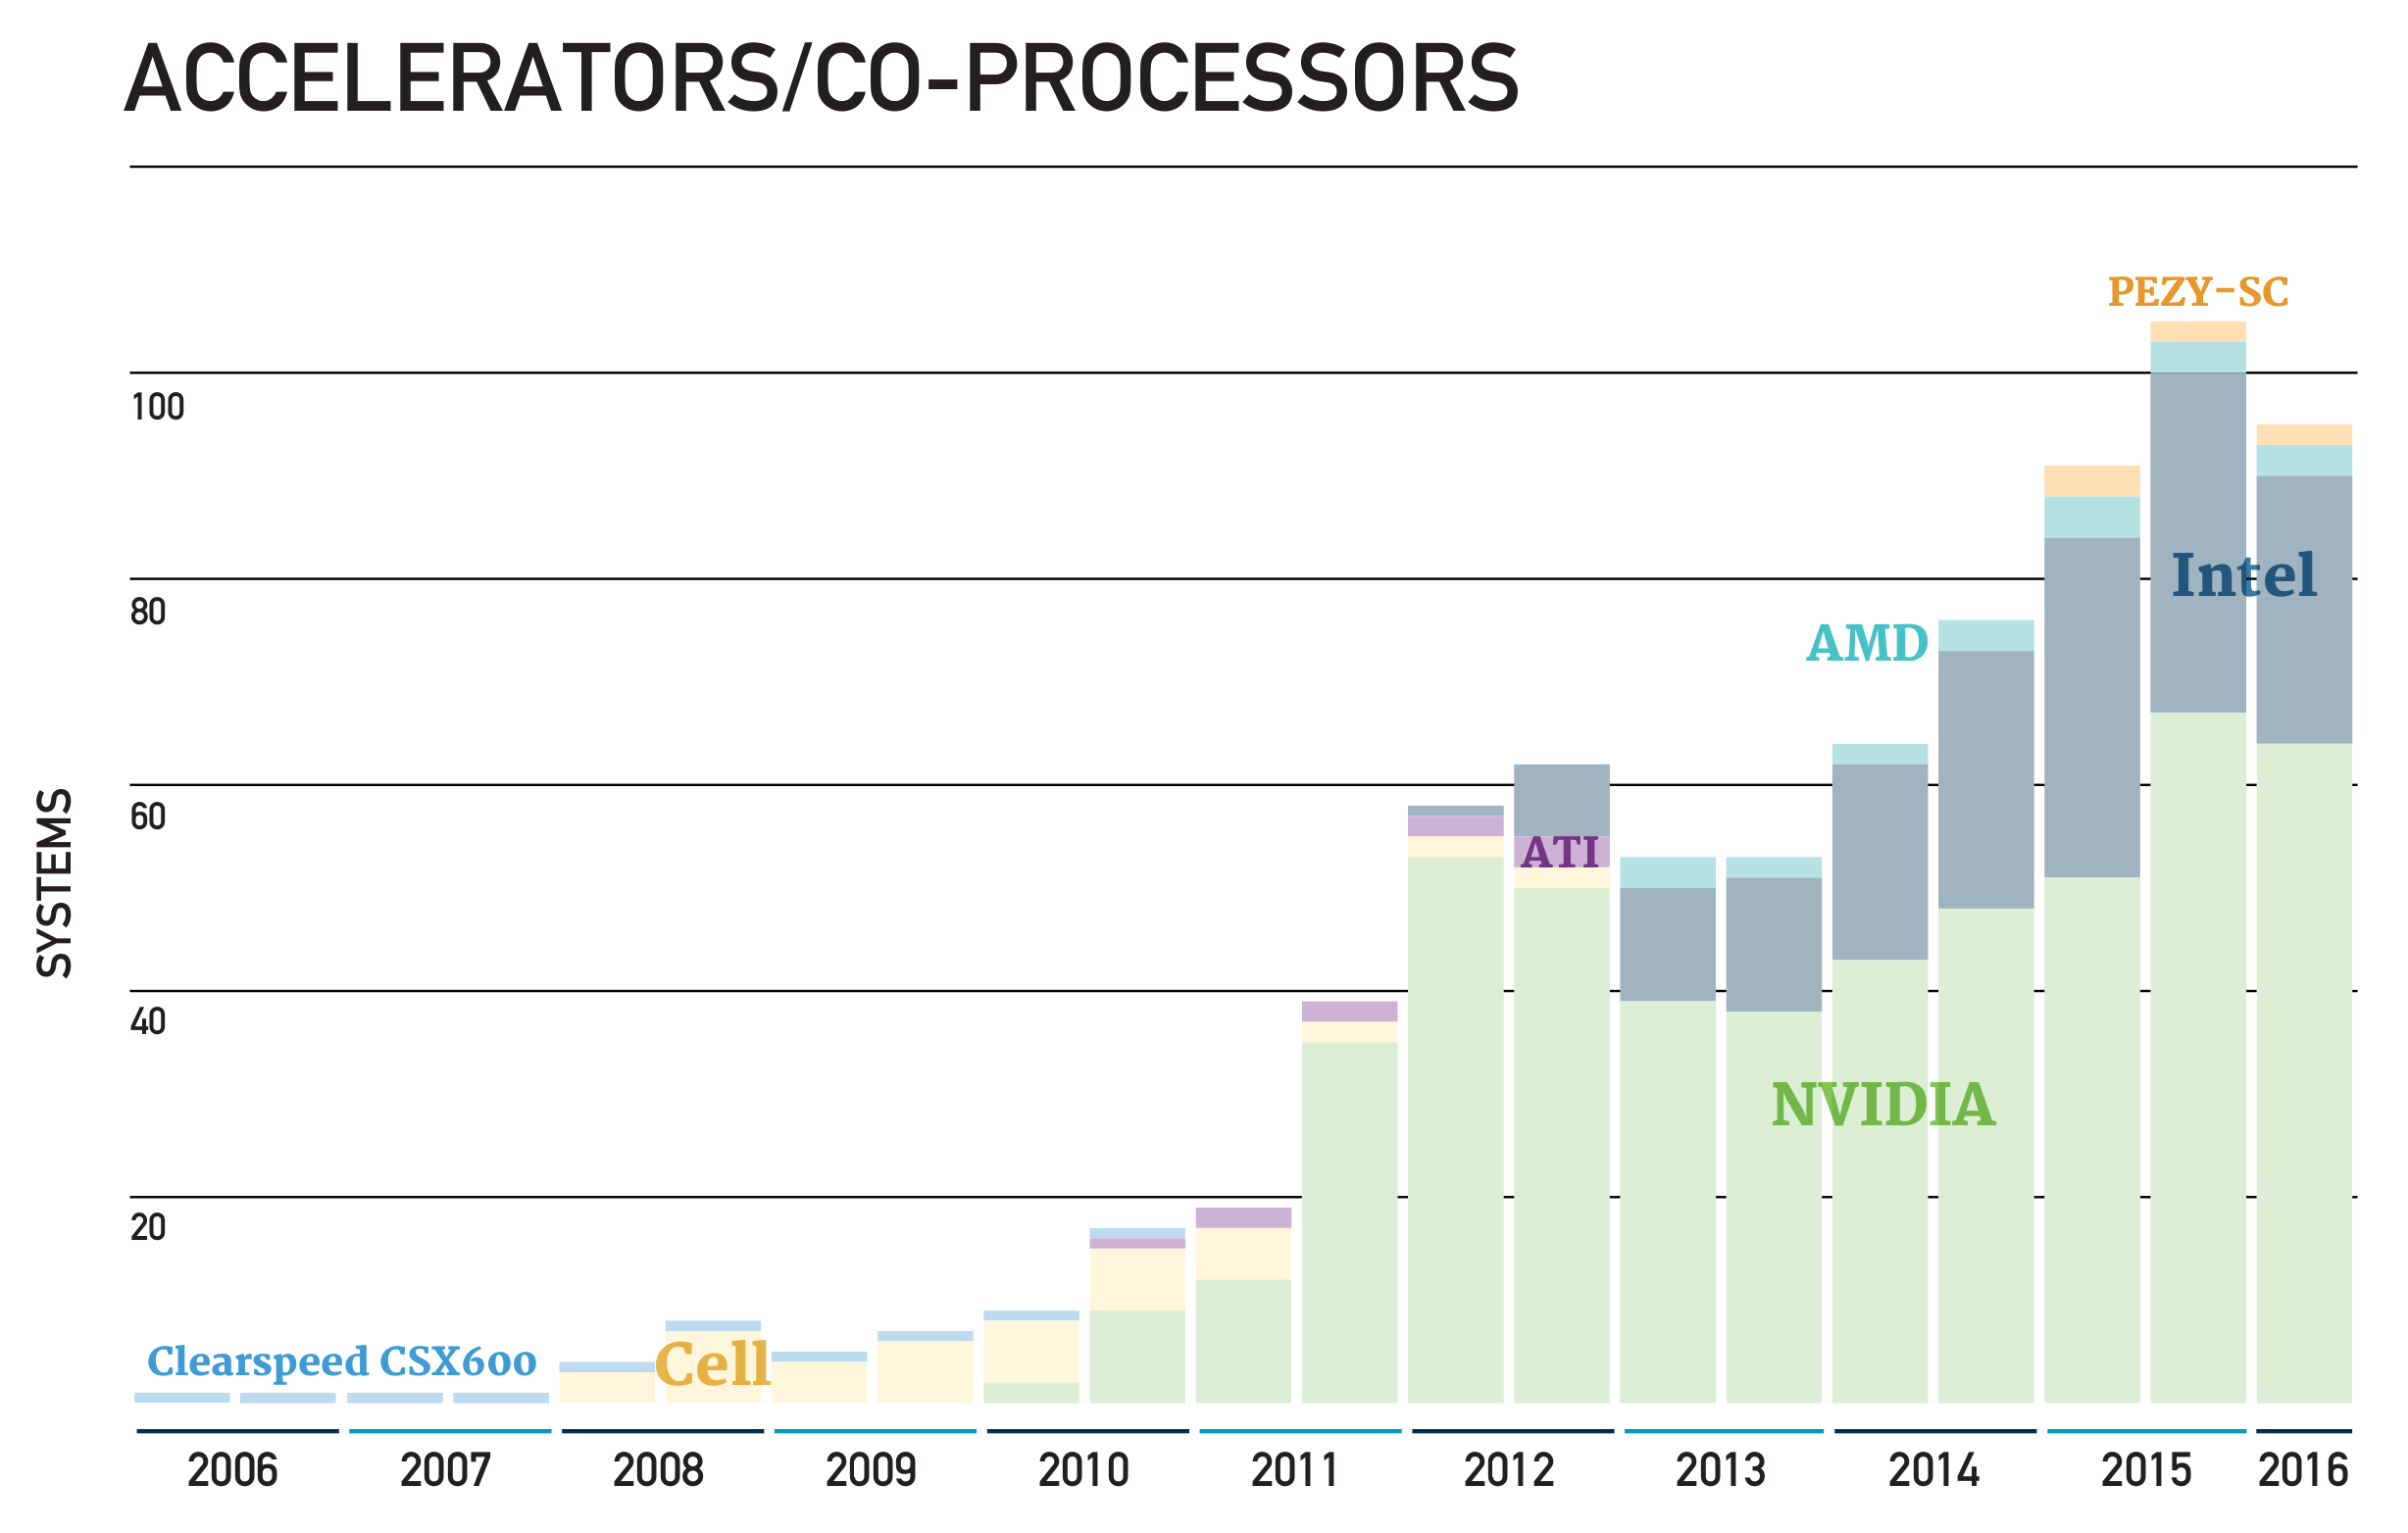
\includegraphics[width=.95\textwidth]{top500_accel}
    \hfill

        \tiny{Image: \url{top500.org/lists/2016/06/download/TOP500_201606_Poster.pdf} [Accessed in 29/07/16]}
    \end{center}
\end{frame}

\begin{frame}
    \frametitle{CUDA C}
    \begin{center}
        
\includegraphics[width=.3\textwidth]{cuda-c}
    \end{center}

    Programming Model:

    \begin{itemize}
        \item \alert{Kernels}
        \item \alert{Threads} hierarchy
        \item \alert{Memory} hierarchy
        \item \alert{Heterogeneous} Programming
    \end{itemize}
\end{frame}

\begin{frame}
    \frametitle{CUDA Libraries}
    \centering
    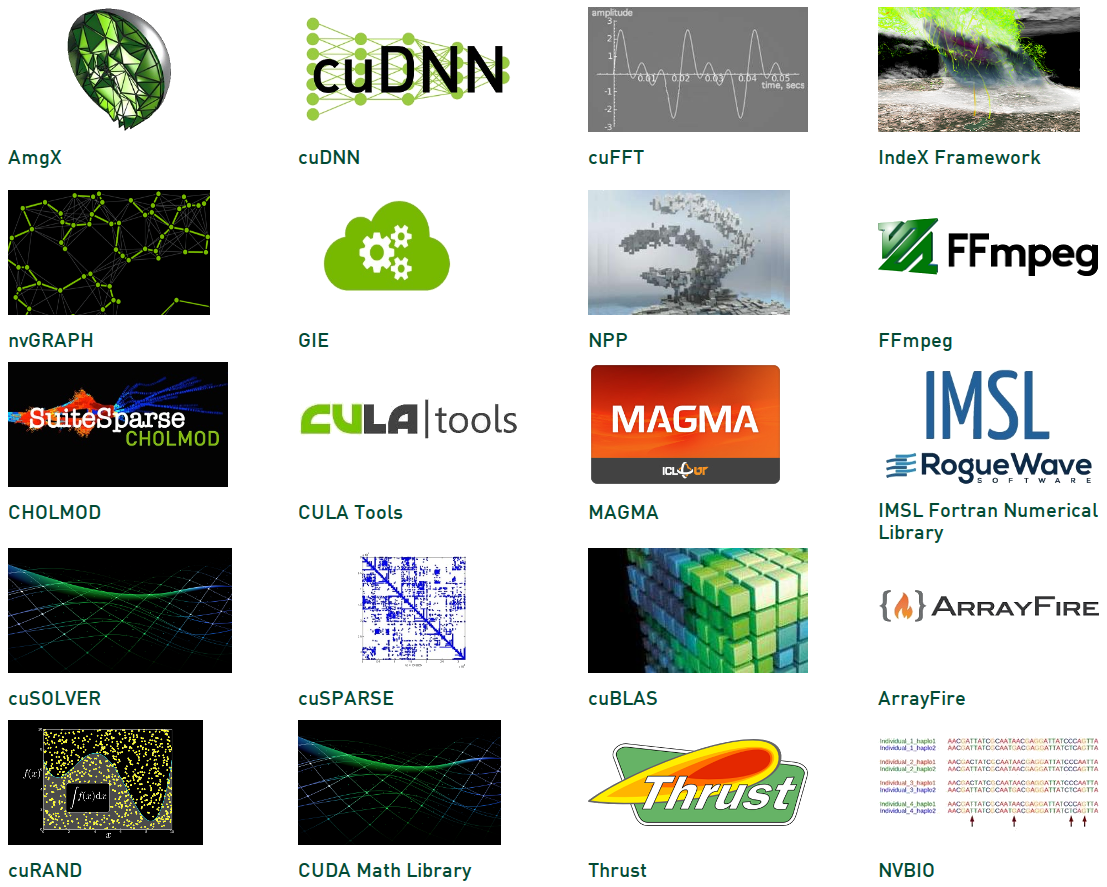
\includegraphics[width=.9\textwidth]{accel_libs_no}
    \vfill

    \tiny{Image: \url{developer.nvidia.com/gpu-accelerated-libraries} [Accessed in 29/07/16]}
\end{frame}

\subsection{Summary}

\begin{frame}
    \frametitle{The Lab: Part I}
    \setbeamertemplate{section in toc}[sections numbered]
    \tableofcontents[hideallsubsections, part=1]
\end{frame}

\begin{frame}
    \frametitle{The Lab: Part II}
    \setbeamertemplate{section in toc}[sections numbered]
    \tableofcontents[hideallsubsections, part=2]
\end{frame}

\section{Heterogeneous Computing}

\section{GPUs}

\section{CUDA Platform}

\section{CUDA C}

\part{Part II}

\section{Recapitulation}

\section{Compiling CUDA Applications}

\section{Optimization Best Practices}

\section{Analysing CUDA Applications}

\section{Otimizing CUDA Applications}

\section{Conclusion}

\subsection{Resources}

\begin{frame}
    \frametitle{Resources}
    This presentation and all source code are available
    at \alert{GitHub}:

    \begin{itemize}
        \item \url{github.com/phrb/intro-cuda}
    \end{itemize}

    More resources:

    \begin{itemize}
        \item CUDA C: \url{docs.nvidia.com/cuda/cuda-c-programming-guide}
        \item CUDA Toolkit: \url{developer.nvidia.com/cuda-toolkit}
        \item Best Practices Guide:
            \begin{itemize}
                \item \url{docs.nvidia.com/cuda/cuda-c-best-practices-guide}
            \end{itemize}
        \item GPU Teaching Kit: \url{syllabus.gputeachingkit.com}
        \item iPython: \url{ipython.org/notebook.html}
        \item Anaconda: \url{continuum.io/downloads}
    \end{itemize}
\end{frame}

\maketitle

\end{document}
